%%%%%%%%%%%%%%%%%%%%%%%%%%%%%%%%%%%%%%%%%
% Journal Article
% LaTeX Template
% Version 1.4 (15/5/16)
%
% This template has been downloaded from:
% http://www.LaTeXTemplates.com
%
% Original author:
% Frits Wenneker (http://www.howtotex.com) with extensive modifications by
% Vel (vel@LaTeXTemplates.com)
%
% License:
% CC BY-NC-SA 3.0 (http://creativecommons.org/licenses/by-nc-sa/3.0/)
%
%%%%%%%%%%%%%%%%%%%%%%%%%%%%%%%%%%%%%%%%%

%----------------------------------------------------------------------------------------
%	PACKAGES AND OTHER DOCUMENT CONFIGURATIONS
%----------------------------------------------------------------------------------------
%for images

% /\/\/\/\/\/\/\/\/\/\/\/\/\/\/\/\/\/\/\/\/\/\/\/\/\/\/\/\/\/\/\/\/\/\/\/\/\/\/\
%
% THIS IS IMPORTANT! RUN WITH pdflatex -shell-escape TO AVOID EPS CONVERSION ERROR
%
% /\/\/\/\/\/\/\/\/\/\/\/\/\/\/\/\/\/\/\/\/\/\/\/\/\/\/\/\/\/\/\/\/\/\/\/\/\/\/\

\documentclass[twoside,twocolumn]{article}

\usepackage{graphicx}

\graphicspath{ {../img/} } 

\usepackage{subfig}
\usepackage{todonotes}
\usepackage[sc]{mathpazo} % Use the Palatino font
\usepackage[T1]{fontenc} % Use 8-bit encoding that has 256 glyphs
\linespread{1.05} % Line spacing - Palatino needs more space between lines
\usepackage{microtype} % Slightly tweak font spacing for aesthetics
\usepackage[english]{babel} % Language hyphenation and typographical rules
\usepackage[hmarginratio=1:1,top=32mm,columnsep=20pt]{geometry} % Document margins
\usepackage[labelfont={bf,up},textfont={it,up}]{caption} % Custom captions under/above floats in tables or figures
\usepackage{booktabs} % Horizontal rules in tables
\usepackage{lettrine} % The lettrine is the first enlarged letter at the beginning of the text

\usepackage{enumitem} % Customized lists
\setlist[itemize]{noitemsep} % Make itemize lists more compact

\usepackage{abstract} % Allows abstract customization
\renewcommand{\abstractnamefont}{\normalfont\bfseries} % Set the "Abstract" text to bold
\renewcommand{\abstracttextfont}{\normalfont\small\itshape} % Set the abstract itself to small italic text

\usepackage{titlesec} % Allows customization of titles
\renewcommand\thesection{\Roman{section}} % Roman numerals for the sections
\renewcommand\thesubsection{\roman{subsection}} % roman numerals for subsections
\titleformat{\section}[block]{\large\scshape\centering}{\thesection.}{1em}{} % Change the look of the section titles
\titleformat{\subsection}[block]{\large}{\thesubsection.}{1em}{} % Change the look of the section titles

\usepackage{fancyhdr} % Headers and footers
\pagestyle{fancy} % All pages have headers and footers
\fancyhead{} % Blank out the default header
\fancyfoot{} % Blank out the default footer
\fancyhead[C]{Bird simulation $\bullet$ \today $\bullet$ v1} % Custom header text
\fancyfoot[RO,LE]{\thepage} % Custom footer text

\usepackage{titling} % Customizing the title section
\usepackage{hyperref} % For hyperlinks in the PDF
\usepackage{amssymb,amsmath,bbold,braket}

%----------------------------------------------------------------------------------------
%	TITLE SECTION
%----------------------------------------------------------------------------------------

\setlength{\droptitle}{-4\baselineskip} % Move the title up

\pretitle{\begin{center}\Huge\bfseries} % Article title formatting
\posttitle{\end{center}} % Article title closing formatting
\title{Simulating a flock of birds} %Simulating a flock of birds
\author{%
\textsc{Steffen Randrup, Michel Smola, Andrei Timus}\\[1ex] % Your name
\normalsize University of Copenhagen \\ % Your institution
%\normalsize \href{mailto:john@smith.com}{john@smith.com} % Your email address
%\and % Uncomment if 2 authors are required, duplicate these 4 lines if more
%\textsc{Jane Smith}\thanks{Corresponding author} \\[1ex] % Second author's name
%\normalsize University of Utah \\ % Second author's institution
%\normalsize \href{mailto:jane@smith.com}{jane@smith.com} % Second author's email address
}
\date{\today} % Leave empty to omit a date
\renewcommand{\maketitlehookd}{%
\begin{abstract}
\noindent
The motion of a flock of birds appears complex and difficult to classify due to
the large number of paticipants each with their own idea of where to go.
Yet such flocks display clear collective motion. In this paper we describe such a flock
similar to a system of self-driven particles interacting with nearby neighbours.
We extend this model by reducing the interaction of any given bird by only interacting with other birds
within the bird's vision. Any bird will act as an average of any other birds it can see.
We show that this simple model of limited interaction may cause the flock to align
over distances larger than the extend of a single bird's interaction. Including how
the noise in each bird's direction and density of birds affect the alignment.
We compare the transition from unordered to ordered motion to a phase transition and
comment on how a vision based approach cause triangular groupings similar to those of migratory birds.
\end{abstract}
}

%----------------------------------------------------------------------------------------

\begin{document}
\maketitle

%----------------------------------------------------------------------------------------
%	ARTICLE CONTENTS
%----------------------------------------------------------------------------------------

\section{Collective motion of birds}

One may consider the collective movement of birds to be described by a simple set of rules.
In this paper we describe the movement of such a flock as a system of self-driven particles.
Our model is an extension of the model presented by Tamás Vicsek and his group in their paper ``Novel Type of Phase Transition in a System of Self-Driven Particles''~\cite{Vicsek}.
The motion of each bird or particle is governed by the motion of other birds or particles nearby.

In our setup the birds were distributed randomly in a square lattice of size $L$.
Each bird had assigned a random direction $\theta$ and a constant interaction radius $r$.
One update consisted of modifying the position of all birds according to the following equation:


\begin{equation}
x_{i}(t+1)=x_i(t)+v_i(t)\Delta t
\end{equation}

where $\Delta$t represents the time between 2 updates.
The velocity of a bird had a constant absolute value and a direction given by:

\begin{equation}
\theta(t+1)=\braket{\theta(t)}_r+\Delta \theta
\end{equation} 

where 

\begin{equation}
  \braket{\theta(t)}_r=\arctan\frac{\braket{\sin(\theta(t))}_r}{\braket{\cos(\theta(t))}_r}
\end{equation}
%
is the average direction of the velocities of nearby birds wich are inside the radius of influence, $r$, of the given bird.
$\Delta \theta$ represents the noise in the system and takes values with equal probability within the interval $[-\eta/2,\eta/2]$.
For a constant number of birds there are 3 parameters which can be varied: $\eta$,$\rho$,and $v$,
where $v$ is the distance a bird travels between 2 updates. This taken as a fixed value of 0.03 as recommended by~\cite{Vicsek}.
$\eta$ describes the interval in which $\Delta\theta$ is picked. $\rho$ is the density of the birds.
This is effectively a way of controlling the size of the lattice if the number of birds is fixed.


We further extend the model by implementing a cone-like vision. This means, that 
rather than averaging the velocities over all birds within a certian radius, we 
only look at a slice of this circle. For a bird to be within the vision of 
another bird, it must be within the interaction radius, $r$, and the angle 
between the bird's velocity and direction to the other bird must be within $\pm \theta_{\text{cone}}$. The 
limit $\theta_{\text{cone}} = \pi$ equals the case without limiting the
cone vision and reproduces the results from~\cite{Vicsek}.

\begin{figure}[!htb]
	\centering
	\subfloat{{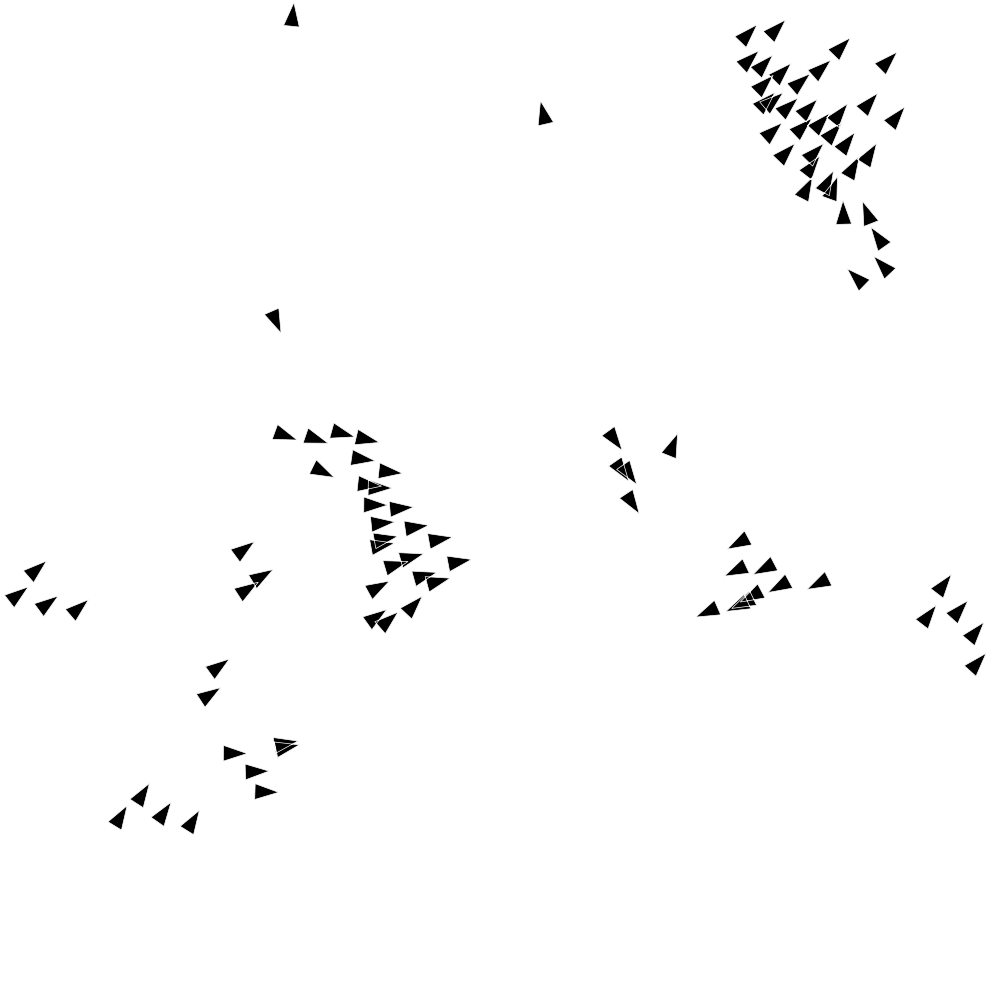
\includegraphics[width=\columnwidth/2]{low-eta-low-rho}}}
  \subfloat{{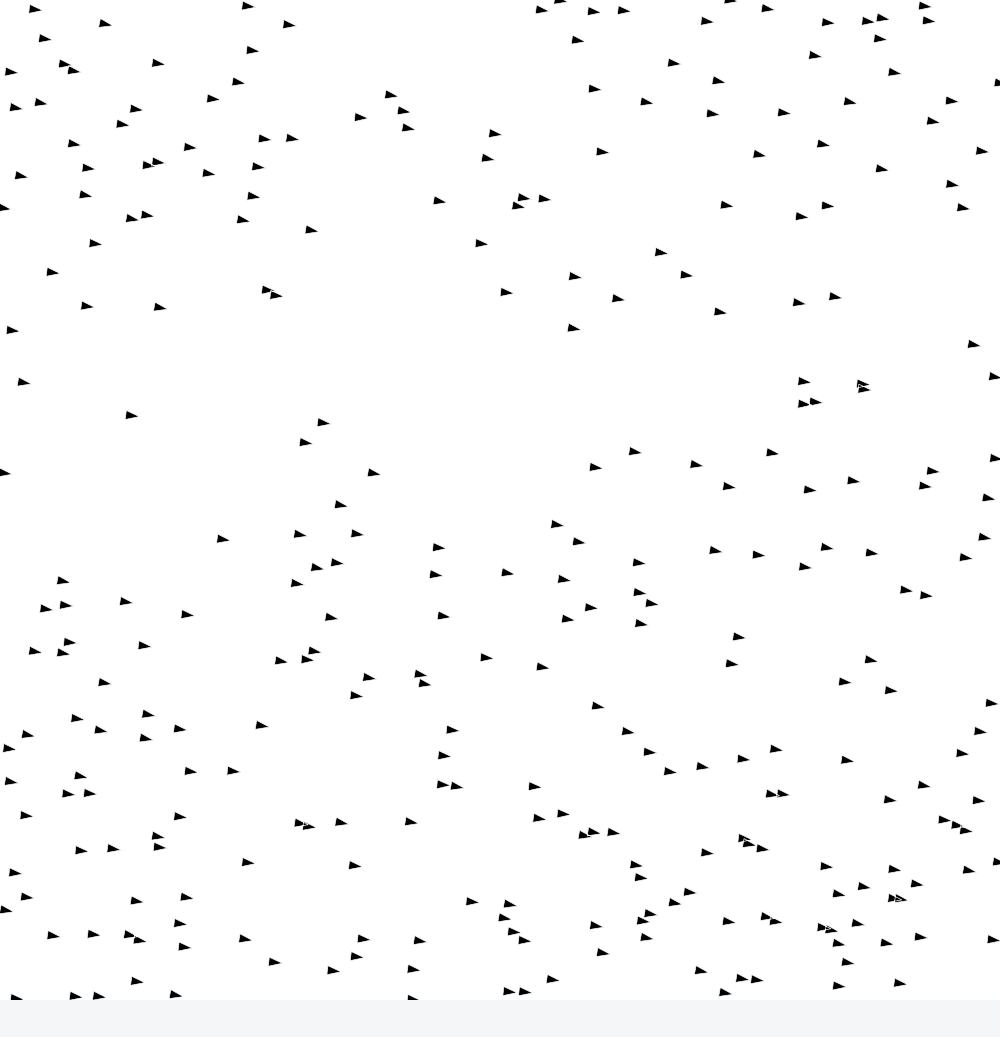
\includegraphics[width=\columnwidth/2]{low-eta-high-rho}}}
	\qquad
	\subfloat{{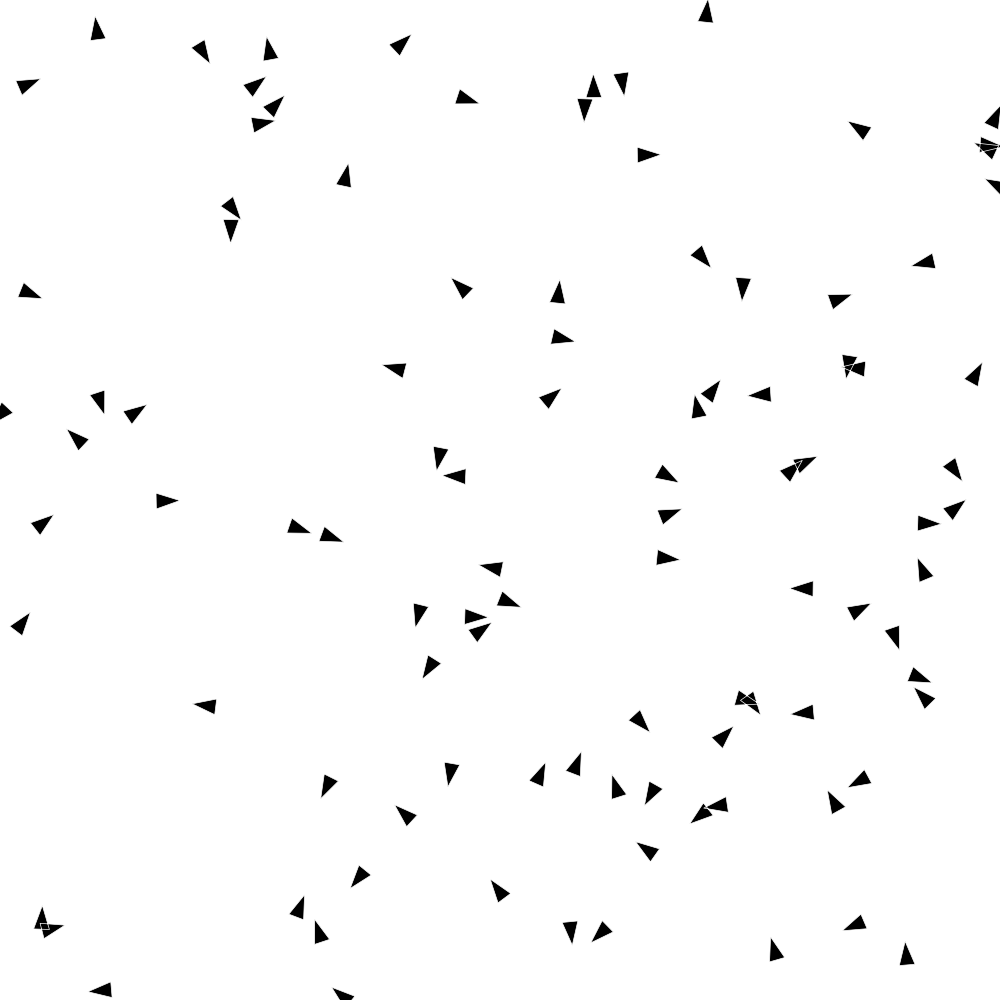
\includegraphics[width=\columnwidth/2]{high-eta-low-rho}}}
	\subfloat{{
\includegraphics[width=\columnwidth/2]{high-eta-high-rho}}}
	\caption{Different configurations of $\eta$ and $\rho$\\Top left: low $\eta$ low $\rho$\\Top right: Low $\eta$, high $\rho$\\Bottm left: High $\eta$, low $\rho$\\Bottom right: High $\eta$, high $\rho$}\label{fig:configs}
\end{figure}

Figure~\ref{fig:configs} shows the configuration of birds for different values of $\rho$ and $\eta$. $\theta_{cone}$ is kept at $\pi$.
For low values of both $\rho$ and $\eta$ the birds tend to form smaller groups in which the birds move in the same direction.
The groups themselves move randomly.
When the noise is high and the density low, the overall motion of the birds is just random.
In the case of high noise and high density, the birds appear to move randomly but with an overall trend in directions
shared among the all the birds.
If the density is high enough, while the noise has low values, the birds move orderly in one direction.
This overall trend in motion is similar to the system going through a kinetic phase transition
where all the particles share the same direction. In order to characterize the behaviour of the flock
we have determined the average normalized velocity of the system and investigated how it changes when the input parameters are modified:

\begin{equation}
v_a=\frac{1}{Nv}\left\vert\sum_{i=1}^{N} v_i\right\vert
\end{equation}

For disordered motion $v_a$ is aproximatively 0, whereas for ordered motion $v_a$ takes on a value near 1.
In our calculations the values of $v_a$ have been taken as a time average after some transient time after which the system has settled into a state, which doesn't change significantly.


The behaviour of $v_a$ is found to be similar to that of the order parameter of some equilibrium systems close to their critical point(like for example the magnetization in the 2D Ising model) if the density is high enough (Fig.2).
If the density is too low the system doesn't reach the disordered state where $v_a\approx 0$ or in other words it doesn't go through a phase transition.In our case the noise and density played the role of a temperature-like variable. Equations~\eqref{eq:va-eta} and~\eqref{eq:va-rho} may be used to describe such a system near the critical value, at which the phase transition occours. 


To determine the critical noise parameter $\eta_c$ we used a quadratic fit model
to to fit the falling curve for $\eta < \eta_c$ and a linear fit for $\eta > 
\eta_c$, both visible in figure~\ref{fig:va_over_eta}. $\eta_c$ is then set to 
the intersection of the fit curves. Hereby we determine $\eta_c = 4.25$


\begin{equation}
  \label{eq:va-eta}
  v_a \approx{[\eta_c(\rho)-\eta]}^\beta 
\end{equation}
\begin{equation}
  \label{eq:va-rho}
  v_a \approx{\left[\rho-\rho_c (\eta)\right]}^\gamma
\end{equation}



% \section{Results}
\section{From disorder to order}

The alignment, $v_a$, depends on the amount of noise $\eta$ in the system 
and the density $\rho$, as seen in equations~\eqref{eq:va-eta} and~\eqref{eq:va-rho}.
In figure~\ref{fig:va_over_eta} we see how the alignment of 
the birds decreases as the randomness of their motion increases. The decrease 
is to be expected, as a higher degree of noise should disrupt alignment. 
This reflects to $v_a$, which approaches $0$ in a totally unordered state and $1$
in a totally ordered state.
What might be more interesting is the general shape of the curves as they as mentioned are similar to
that of a phase transition. We may then 
determine $\beta$ from equation~\eqref{eq:va-eta} to be 0.57 for $N=400$. This is also shown in figure~\ref{fig:criticaleta}. The results presented here 
are all computed without the conevision (equivalent to $\theta_{\text{cone}} = \pi$). 
Figure~\ref{fig:va_over_eta} shows how $v_a$ varies with the noise $\eta$ and 
density $\rho$ for a constant value of density and noise respectively.
As seen in Figure~\ref{fig:va_over_eta} the overall alignment of the birds depends 
on the noise and for a high number of birds N the system becomes less ordered. 
For low $\eta$ the flock reaches a coherent moving phase, while for high $\eta$ 
the birds move randomly in the lattice.  


\begin{figure}[!htb]
  \centering
  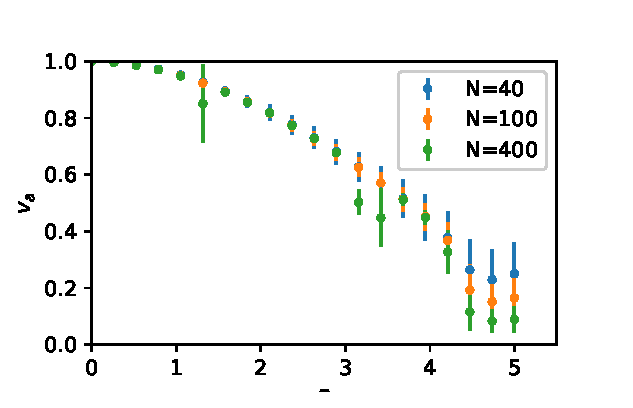
\includegraphics[width=\columnwidth]{va_over_eta}
  \caption{Dependance of alignment on randomness}\label{fig:va_over_eta}
\end{figure}


\begin{figure}[!htb]
	\centering
	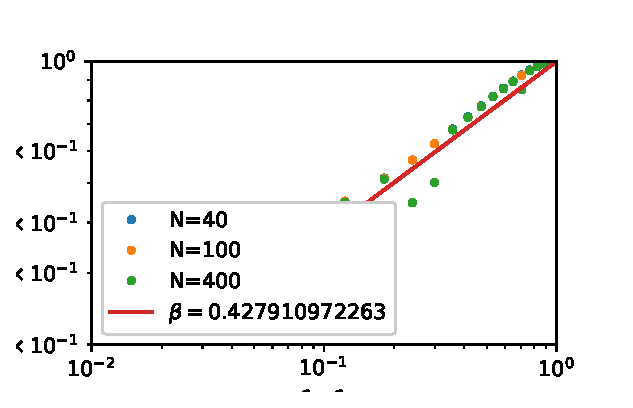
\includegraphics[width=\columnwidth]{va_over_etac_minus_eta_over_etac}
	\caption{Determining $\beta$}\label{fig:criticaleta}
\end{figure}

Similarly we may see the effects of the density on the alignment of birds. This also fits the prediction from equation~\eqref{eq:va-rho}. This is shown in figure~\ref{fig:va_over_rho}.

\begin{figure}[!htb]
	\centering
	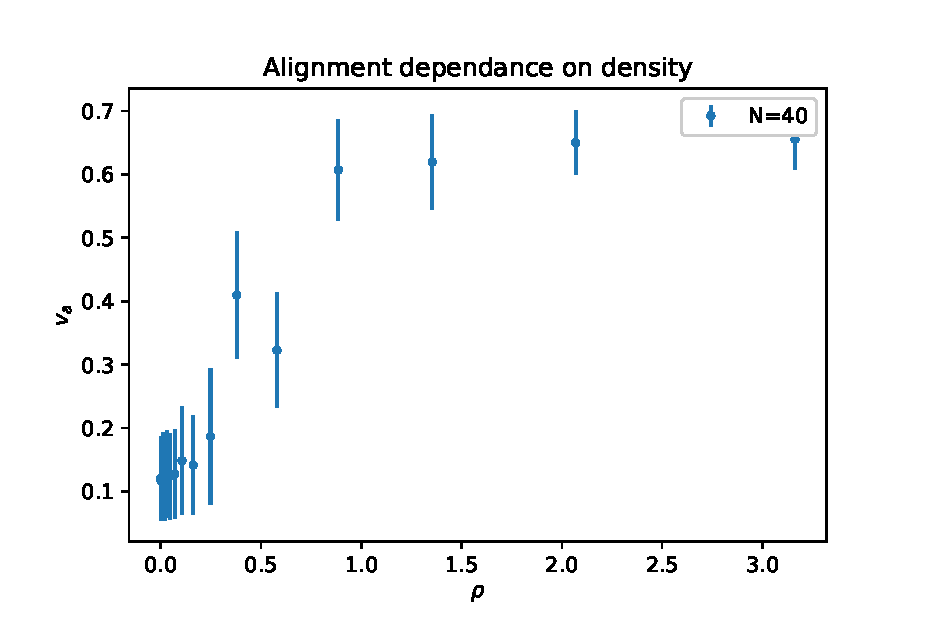
\includegraphics[width=\columnwidth]{va_over_rho}
	\caption{Dependance of alignment on density}\label{fig:va_over_rho}
\end{figure}

\subsection*{Cone-like vision}\label{subsec:conevision}

The cone-like vision has little effect on the final alignment of the birds.
The effect only becomes apparent near the critical value of $\rho=0.1$ after which
the alignment increases dramatically as shown in Figure~\ref{fig:va_over_rho}.
In Figure~\ref{fig:conevision} we see how only the configuration with $\rho$ near the
transition between the unordered and ordered states is affected by the implementation of the vision.
There is as expected a slight upward trend in alignment as the angle of the vision is increased.
A much more interesting result is the shape of the formed groups. In stead of forming
dense groups, the birds now form lines or open triangles whose shapes are defined
by the angle of vision. An example of such a configuration is seen in Figure~\ref{fig:angle-birds}.


\begin{figure}[!htb]
\begin{center}
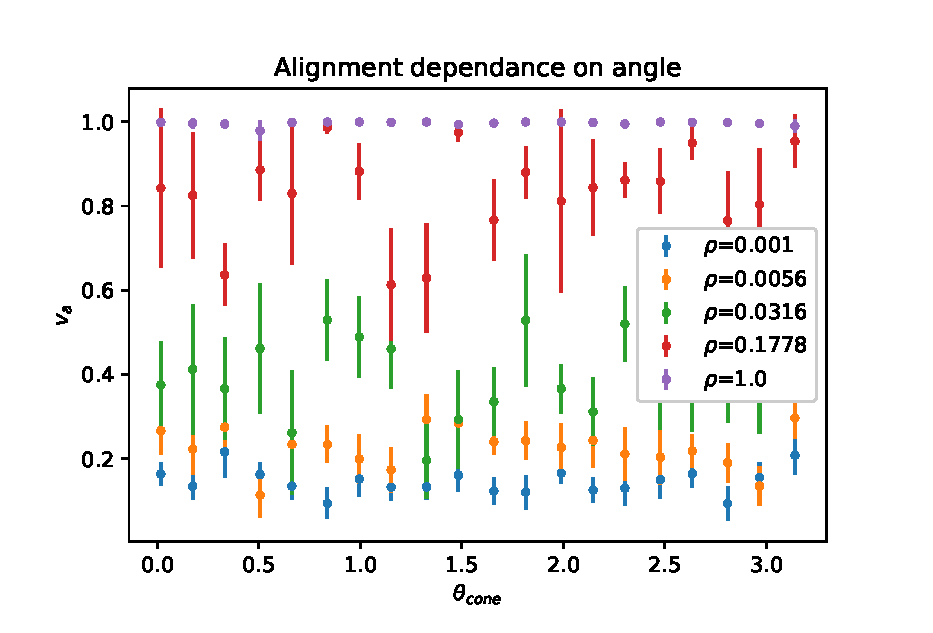
\includegraphics[width=\columnwidth]{va_over_angle}
\end{center}
\caption{The effect of the cone vision is only visible for adequately small densities}\label{fig:conevision}
\end{figure}

\begin{figure}[!htb]
\begin{center}
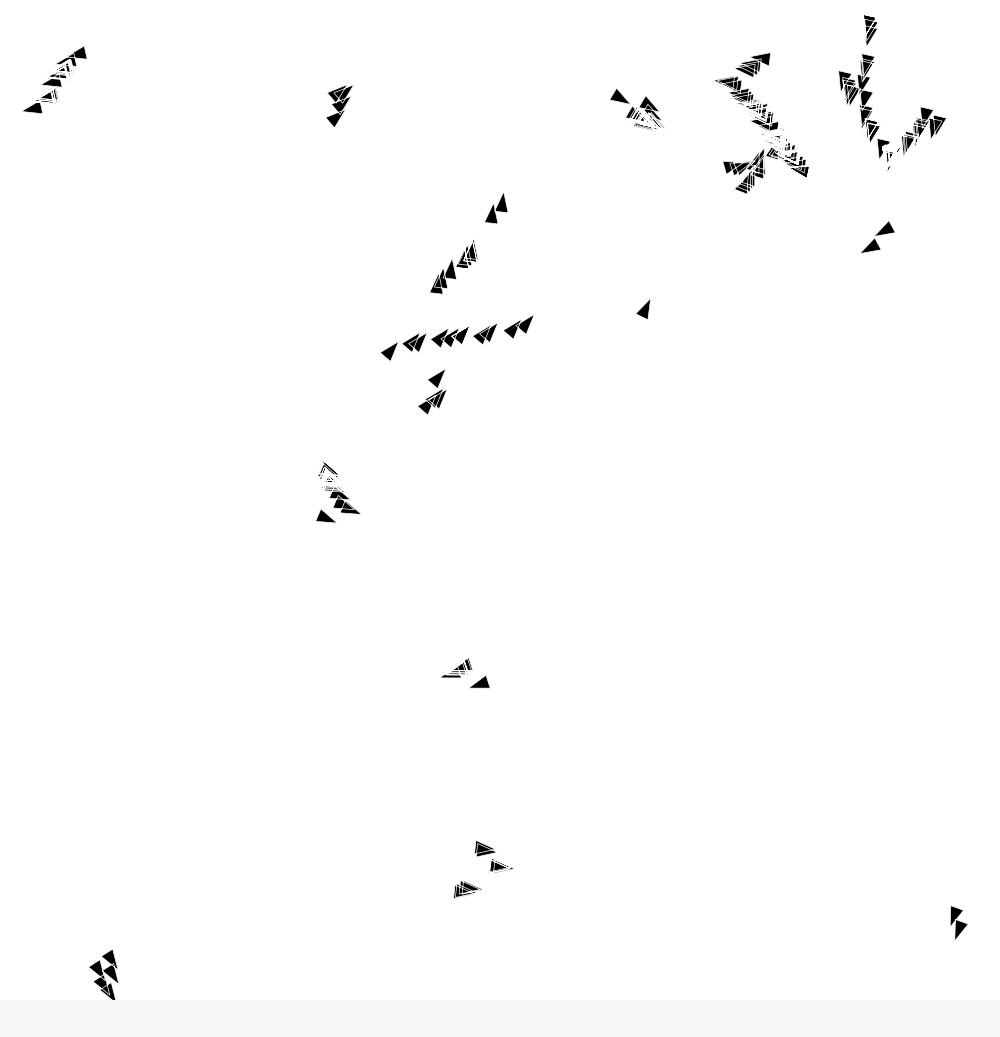
\includegraphics[width=\columnwidth]{angles}
\end{center}
\caption{Birds form lines or triangular groups when a cone-like vision is implemented and the density is low}\label{fig:angle-birds}
\end{figure}

\section{Discussion}

The shape of the formed groups when implementing the cone-like vision was a surprising result.
The triangular shape is commonly seen in migratory birds but is usually ascribed to other factors.
Our simpel model of simply letting the birds do as other birds within their sight reproduces this
effect. It is easily explained by considering two birds. One approaches the other from the side.
The first bird will see the other and follow it, whereas the second bird will see nothing and just
continue. In this way the birds form a line. If birds approach from the other side, they will line
up in a similar fashion causing a combined triangular shape. Once a traingle has formed it is much
more likely for a new approaching bird to align with one of the sides of the trangle rather than
joining the group somewhere else. In this way the triangles keep growing.
That the effect on alignment is only detectable in a limited range also makes sense, because for
low densities, it will be unlikely for birds to come close enough to each other to form groups.
For higher densities there will more often be a bird within any other bird's vision. This causes
larger, coherent groups to form.


\section{Conclusion}


In this paper we have presented a model for studying the motion of a flock of birds.
The model contained contained few variables; density of birds, noise in their direction and an angle
controlling which other birds influence a given bird's motion. Each of these variables gave rise
to the movement of the flock going between disordered and ordered. For the case of the angle based
vision the effects on alignment was only detectable near the transition between the unordered
and ordered state for the density of birds.
However the vision based approach gave rise to different shapes of the groups formed when the density
was sufficiently low. When the vision approach was not used, the groups were dense and clumped
together. When the vision was implemented, the birds formed lines or triangular groups.



%----------------------------------------------------------------------------------------
%	REFERENCE LIST
%----------------------------------------------------------------------------------------

\begin{thebibliography}{99} % Bibliography - this is intentionally simple in this template

  \bibitem{Vicsek}Tamás Vicsek, András Czirók, Eshel Ben-Jacob, Inon Cohen and Ofer Shochet\\
  Novel Type of Phase Transition in a System of Self-Driven Particles\\
  Physical Review Letters, Volume 75, Number 6, August 1995
 
\end{thebibliography}

%----------------------------------------------------------------------------------------

\end{document}
